\let\negmedspace\undefined
\let\negthickspace\undefined
\documentclass[journal]{IEEEtran}
\usepackage[a5paper, margin=10mm, onecolumn]{geometry}
%\usepackage{lmodern} % Ensure lmodern is loaded for pdflatex
\usepackage{tfrupee} % Include tfrupee package

\setlength{\headheight}{1cm} % Set the height of the header box
\setlength{\headsep}{0mm}     % Set the distance between the header box and the top of the text

\usepackage{gvv-book}
\usepackage{gvv}
\usepackage{cite}
\usepackage{amsmath,amssymb,amsfonts,amsthm}
\usepackage{algorithmic}
\usepackage{graphicx}
\usepackage{textcomp}
\usepackage{xcolor}
\usepackage{txfonts}
\usepackage{listings}
\usepackage{enumitem}
\usepackage{mathtools}
\usepackage{gensymb}
\usepackage{comment}
\usepackage[breaklinks=true]{hyperref}
\usepackage{tkz-euclide} 
\usepackage{listings}
\usepackage{gvv}                                        
\def\inputGnumericTable{}                                 
\usepackage[latin1]{inputenc}                                
\usepackage{color}                                            
\usepackage{array}                                            
\usepackage{longtable}                                       
\usepackage{calc}                                             
\usepackage{multirow}                                         
\usepackage{hhline}                                           
\usepackage{ifthen}                                           
\usepackage{lscape}
\usepackage{circuitikz}
\tikzstyle{block} = [rectangle, draw, fill=blue!20, 
    text width=4em, text centered, rounded corners, minimum height=3em]
\tikzstyle{sum} = [draw, fill=blue!10, circle, minimum size=1cm, node distance=1.5cm]
\tikzstyle{input} = [coordinate]
\tikzstyle{output} = [coordinate]


\begin{document}

\bibliographystyle{IEEEtran}
\vspace{3cm}

\title{2.5.3}
\author{EE25BTECH11049 - Sai Krishna Bakki}
 \maketitle
% \newpage
% \bigskip
{\let\newpage\relax\maketitle}

\renewcommand{\thefigure}{\theenumi}
\renewcommand{\thetable}{\theenumi}
\setlength{\intextsep}{10pt} % Space between text and floats


\numberwithin{equation}{enumi}
\numberwithin{figure}{enumi}
\renewcommand{\thetable}{\theenumi}

\textbf{Question}:\\
Show that the points (-2, 3), (8, 3), and (6, 7) are the vertices of a right-angled triangle. \\ 
\solution \\
Given:
\begin{align}
 \vec{A}=\myvec{-2\\3},
 \vec{B}=\myvec{8\\3},
 \vec{C}=\myvec{6\\7}
\end{align} 
\begin{align}
   \vec{B}-\vec{A}=\myvec{10\\0},
   \vec{C}-\vec{B}=\myvec{-2\\4},
   \vec{C}-\vec{A}=\myvec{8\\4}
\end{align}
For a right angle, the dot product of two sides must be zero,
\begin{align}
\brak{\vec{C}-\vec{A}}^T\brak{\vec{B}-\vec{A}}=\brak{10}\brak{8}+\brak{0}\brak{4}=80\neq 0
\end{align}
\begin{align}
\brak{\vec{B}-\vec{A}}^T\brak{\vec{C}-\vec{B}}=\brak{-2}\brak{10}+\brak{4}\brak{0}=-20\neq 0
\end{align}
\begin{align}
\brak{\vec{C}-\vec{A}}^T\brak{\vec{C}-\vec{B}}=\brak{-2}\brak{8}+\brak{4}\brak{4}=0
\end{align}
Hence $\triangle$ABC is right angled at \textbf{C}.
\newpage
\begin{figure}
    \centering
    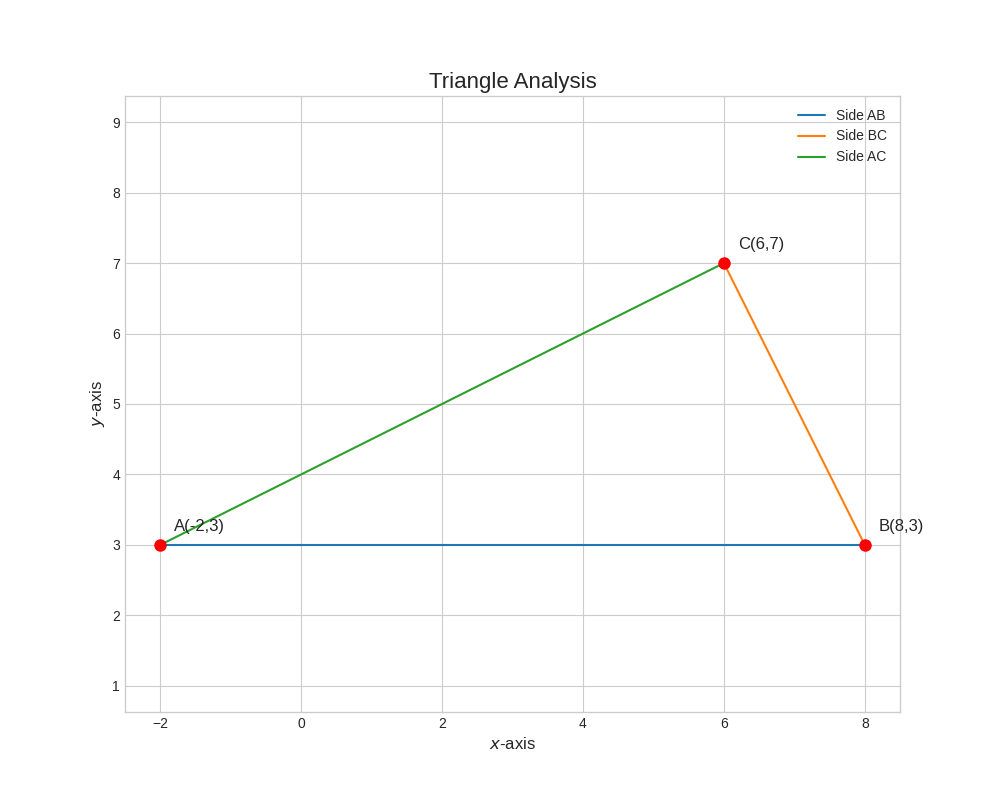
\includegraphics[width=1\columnwidth]{figs/Figure_1.png}
    \caption{}
    \label{fig:placeholder}
\end{figure}


\end{document}